\section{Preliminaries}

\subsection{Semirings}

\paragraph{} A monoid \cite{Golan1999_1} $M = (\mathbb{M}, \odot, e)$ is an algebraic structure over the non-empty set $\mathbb{M}$ with an associative binary function $\odot : \mathbb{M} \times \mathbb{M} \mapsto \mathbb{M}$ whose identity element is $e$, i.e. $(x \odot y) \odot z = x \dot (y \odot z)$ and $e \odot x = x \odot e = x$, $\forall x, y, z \in \mathbb{M}$.  A monoid is commutative is $x \odot y = y \odot x$, $\forall x, y \in \mathbb{M}$

\paragraph{} A semiring \cite{Golan1999_1} $K = (\mathbb{K}, \oplus, \otimes, \bar{0}, \bar{1})$ is an algebraic structure over the non-empty set $\mathbb{K}$ statisfying the following conditions:
\begin{itemize}
    \item $(\mathbb{K}, \oplus, \bar{0})$ is a commutative monoid
    \item $(\mathbb{K}, \otimes, \bar{1})$ is a monoid
    \item $\otimes$ distributes over $\oplus$ from either sides, i.e. $a \otimes (x \oplus y) = (a \otimes x) \oplus (a \otimes y)$ and $(x \oplus y) \otimes a = (x \otimes a) \oplus (y \otimes a)$, $\forall a, x, y \in \mathbb{K}$
    \item $\bar{0} \otimes x = x \otimes \bar{0} = \bar{0}$, $\forall x \in \mathbb{K}$.
\end{itemize}
We say that $K$ is a commutative semiring if $\otimes$ is commutative.

\subsection{Semimodules and $K$-vector space}

Let $K = (\mathbb{K}, \oplus, \otimes, \bar{0}, \bar{1})$ be a semiring. A left $K$-semimodule \cite{Golan1999_2} $S = (\mathbb{S}, K, +, \cdot)$ is a commutative monoid $(
\mathbb{S}, +, \mathbf{0})$ augmented with a function $\cdot : \mathbb{K} \times \mathbb{S} \mapsto \mathbb{S}$, denoted \emph{scalar multiplication} (we write $a \cdot \mathbf{x} = a 
\mathbf{x}$) statisfying the following conditions:
\begin{itemize}
    \item $(a \otimes b) \mathbf{x} = a \otimes (b \mathbf{x})$
    \item $a \otimes (\mathbf{x} + \mathbf{y}) = (a \otimes \mathbf{x}) + (a \otimes \mathbf{y}) $
    \item $(a \oplus b) \mathbf{x} = a \mathbf{x} + b \mathbf{x}$
    \item $\bar{1} \mathbf{x} = \mathbf{x}$
    \item $a \mathbf{0} = \mathbf{0} = \bar{0} \mathbf{x}$,
\end{itemize}
$\forall a, b \in \mathbb{K}$ and $\forall \mathbf{x}, \mathbf{y} \in S$. A right $K$-semimodule follows the same definition with a "right" scalar multiplication.

\paragraph{} Let $K_1$ and $K_2$ be two semirings over the set $\mathbb{K}_1$ and $\mathbb{K}_2$ respectively. We say that $S = (\mathbb{S}, K, +, \cdot)$ is a $(K_1, K_2)$-bisemimodule \cite{Golan1999_2} if $S$ is a left $K_1$-semimodule and a right $K_2$-semimodule and if it satisfies the additional constraint $(a \mathbf{x}) b = a (\mathbf{x} b)$ for all $a \in \mathbb{K}_1$, $\mathbf{x} \in \mathbb{S}$ and $b \in \mathbb{K}_2$.

\paragraph{} We define the $p$-dimensional $K$-vector space as the $(K, K)$-bisemimodule $S = (\mathbb{K}^p, K, +, \cdot)$ constructed as 
\begin{itemize}
    \item $\mathbf{x} + \mathbf{y} = \begin{bmatrix} x_1 \oplus y_1 & \dots & x_d \oplus y_d \end{bmatrix}^\top$, $\forall \mathbf{x}, \mathbf{y} \in \mathbb{K}^p$ 
    \item $a \mathbf{x} = \begin{bmatrix} a \otimes x_1 & \dots & a \otimes x_d \end{bmatrix}^\top$, $\forall a \in \mathbb{K}$ and $\forall \mathbf{x} \in \mathbb{K}^p$.
\end{itemize}
We call an element of $S$ a $K$-\emph{vector}. We define the \emph{dot product}, between two $K$-vectors $\mathbf{x}$ and $\mathbf{y}$, denoted $\mathbf{x}^\top \mathbf{y}$, as 
\begin{align}
    \mathbf{x}^\top \mathbf{y} &= x_1 \otimes y_1 \oplus \dots \oplus x_d \otimes y_d.
\end{align}
Note that the dot product between $K$-vectors is commutative, i.e. $\mathbf{x}^\top \mathbf{y} = \mathbf{y}^\top \mathbf{x}$ only if $K$ is a commutative semiring. 

\paragraph{} The concept of $K$-vector is trivially extended to the one of $K$-matrix (defined over elements of $\mathbb{K}^{p \times q}$). We define the multiplication of a $p \times q$ matrix $\mathbf{A}$ with a $q$-dimensional vector $\mathbf{x}$ as: 
\begin{align}
    \mathbf{A} \mathbf{x} = \mathbf{a}_1 x_1 + \dots + \mathbf{a}_q x_q 
    \label{eq:mv_mul}
\end{align}
where $\mathbf{a}_i$ is the $i$th column of $\mathbf{M}$. Similarly the multiplication of $p$-dimensional transposed $K$-vector $\mathbf{y}^\top$ and a $p \times q$ $K$-matrix $B$ is defined as 
\begin{align}
    \mathbf{y}^\top \mathbf{B} = y_1 \mathbf{b}^1 + \dots + y_p \mathbf{b}^p.
    \label{eq:mvt_mul}
\end{align}
where $\mathbf{b}^i$ is the $i$th row of $\mathbf{B}$. Similarly to the dot product operation, the relation $(\mathbf{A} \mathbf{x})^\top = \mathbf{x}^\top \mathbf{A}^\top$ only holds for all $\mathbf{x} \in \mathbb{K}^q$ if $K$ is a commutative semiring.

\paragraph{} Let $\mathbf{A}$ be a $p \times q$ $K$-matrix, $\mathbf{B}$ a $q \times r$ $K$-matrix. We write the $i$th element of the $j$th column of a ($K$-)matrix $x_j^i$. From \eqref{eq:mv_mul} and $\eqref{eq:mvt_mul}$, we define the $K$-matrix multiplication between $\mathbf{A}$ and $\mathbf{B}$, denoted $\mathbf{A} \mathbf{B}$, the operation producing a $p \times r$ $K$-matrix whose $i$th column is defined as $ \mathbf{a}_1 b_i^1 + \dots + \mathbf{a}_d b_i^d$, or equivalently, whose $j$th row is defined as $a^j_1 \mathbf{b}_1 + \dots + a^j_d \mathbf{b}_d $.

\subsection{Weighted Finite State Automata}

A Weighted Finite State Automaton (WFSA) \cite{Mohri2008} $\mathcal{A} = (\Lambda, Q, I, F, \alpha, \omega, E)$ over a semiring $K$ is a 7-tuple where:
\begin{itemize}
    \item $\Lambda$ is the set of input symbols containing at least the empty sequence $\epsilon$;
    \item $Q$ is the set of states;
    \item $I \subseteq Q$, $F \subseteq Q$ are the sets of initial and final states respectively;
    \item $\alpha : I \mapsto K$, $\omega : F \mapsto K$ are the initial and final weight assignment respectively;
    \item $E \subseteq Q \times \Sigma \times K \times Q$ is a finite set of transitions.
\end{itemize}

\paragraph{} Given transition $e \in E$, $p[e]$ denotes its previous state, $n[e]$ its next state, $w[e]$ its weight and $\lambda[e]$ its label. A path $\boldsymbol{\pi} = e_1 \dots e_k$ is a sequence of transition such that $n[e_{i-1}] = p[e_i]$. We write $|\boldsymbol{\pi}|$ the length of the path, i.e. the number of transitions. The weight of a path $w[\boldsymbol{\pi}] = w[e_1] \otimes \dots \otimes w[e_k]$ is the $\otimes$-product of all its transitions. We say that a string of symbols $\mathbf{x} = x_1 \dots x_k$ is accepted by an automaton $\mathcal{A}$ if there is a path $\boldsymbol{\pi} = e_1 \dots e_l$ in $\mathcal{A}$ with weight $w[\boldsymbol{\pi}] \neq \bar{0}$ such that $\mathbf{x} = \lambda[e_1] \dots \lambda[e_l]$. 

\paragraph{} The weight of an automaton $\mathcal{A}$, denoted $W(\mathcal{A})$, is defined as the $\oplus$-sum of all its accepted path. 

%
\begin{figure}[t] % ’ht’ tells LaTeX to place the figure ’here’ or at the top of the page
    \centering 
    \subcaptionbox{common WFSA.}
        {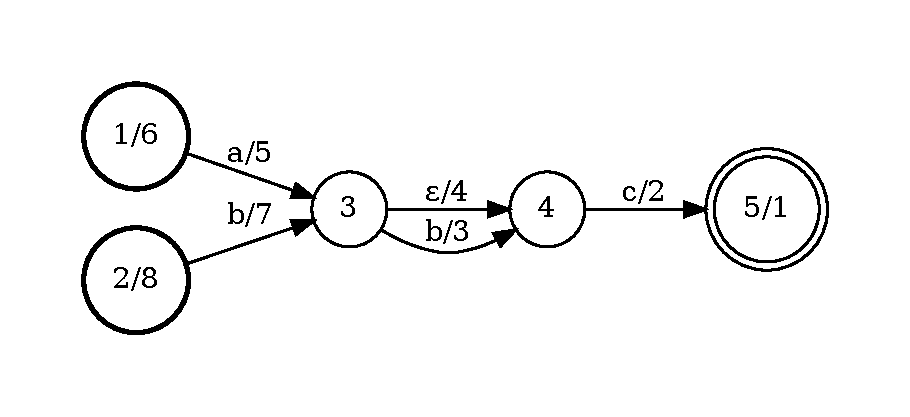
\includegraphics[width=0.7\linewidth]{images/reg_fsa.pdf}}
    \subcaptionbox{\label{simple} simple WFSA.}
        {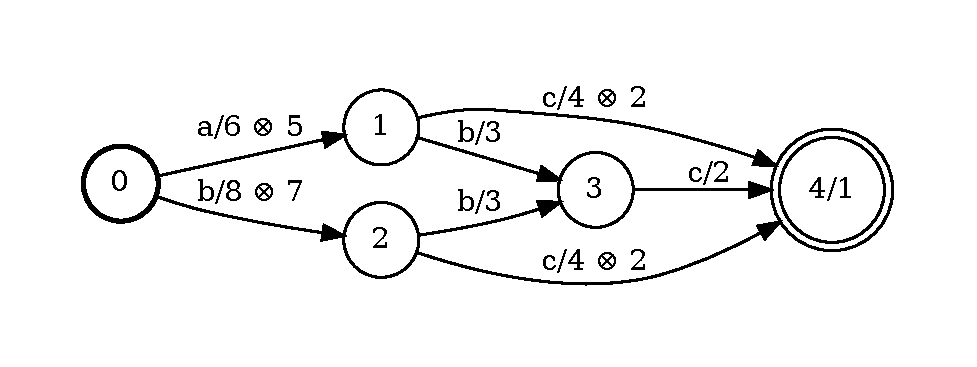
\includegraphics[width=0.7\linewidth]{images/simple_fsa.pdf}}
    \caption{Example of equivalent WFSA accepting the sequences $abc, ac, bbc$, and $bc$.}
    \label{fig:standard_fsa}
\end{figure}